\begin{figure}
\centering
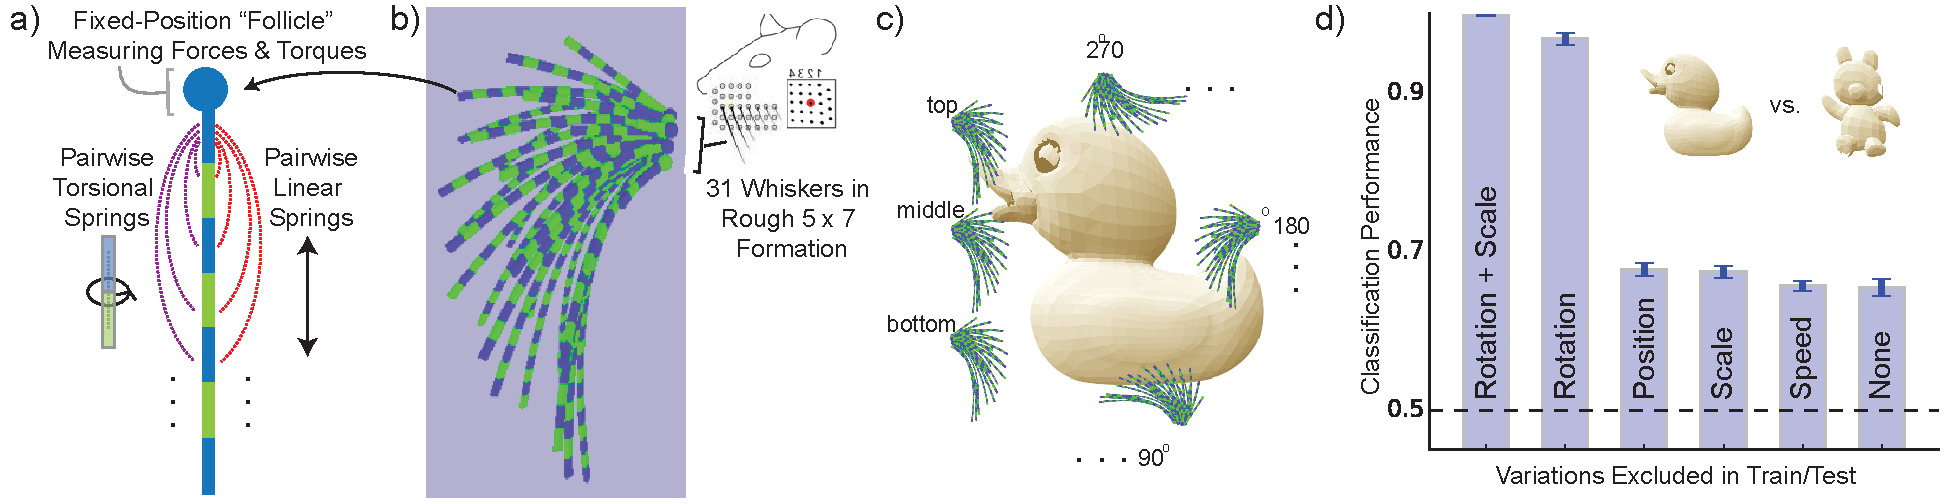
\includegraphics [width=1\linewidth]{figures/whiskers.pdf}
\vspace{-2mm}
\caption{\textbf{Dynamic Three-Dimensional Whisker Model:} \textbf{a.} We constructed an array of 31 whisker objects, arranged in a 5x7 grid (with 4 missing elements).  
Whisker number, placement, length and static shape were matched to biophysical data. 
\textbf{b.} Each whisker element is composed of a set of cuboid objects.  
The follicle cuboid has a fixed location, and is attached to movable cuboids making up the rest of the hair. 
Motion is constrained by linear and torsional springs between each pair of cuboid elements.  
The parameters of these springs are chosen to ensure naturalistic motion of the whiskers.  
\textbf{c.} During dataset construction, the whisker is brought into contact with each object at three vertical heights (top, middle bottom), at each of 4 90-degree separated attack angles, for a total of 12 swipes.  
Object initial angle, size, and swipe speed vary randomly between each group of 12 swipes.
Forces and torques are recorded at the three cuboids closest to to the follicle, for a total of 18 measurements per whisker per timepoint. 
\textbf{d.} Basic validation of performance of binary linear classifier trained on raw sensor output to distinguish between two shapes (in this case, a duck versus a teddybear).  Classifier was trained/tested on several equal-sized datasets in which variation on one or more latent variable axes is been suppressed. ``None'' indicates that all variations are present. Dotted line represents chance performance (50\%).~\label{fig_whiskers}}
\end{figure}

In order to provide our neural networks inputs similar to those of rodent somatosensory systems, we constructed a physically-accurate 3d simulated model of the rodent vibrissal array (Fig. \ref{fig_whiskers}).  
We wanted the the mechanical details of every individual whisker to be correct, but at the same time, also needed simulations to be fast enough to generate a large training dataset.   
We thus used the Bullet~\cite{wiki:bullet}, an open-source real-time physics engine used in many video games. 
To make our model biologically accurate, we incorporated measurements from detailed biophysical studies about whisker number, relative position, length and curvature~\cite{Towal2011}.

\textbf{Statics.} Each individual whisker was modeled as a chain of 2mm cuboid elements, with the number of cuboids constrained to ensure that its length matched that of the corresponding real whisker (Fig. \ref{fig_whiskers} a).
The first cuboid in each simulated whisker, corresponding to the follicle cell at the whisker base where it attaches to the rodents face, was pegged to a fixed 3-dimensional spatial location.  
Each cuboid is also endowed with first-order linear and rotational damping factors to ensure that unforced motions dissipate over time. 
To simplify our model, we assume that the damping factors were shared across all cuboids in a given whisker.  
Within each whisker, each pair of cuboids was connected with linear and torsional first-order springs, each of which has two parameters (equilibrium displacement and stiffness).  
The equilibrium displacements of each spring were chosen to ensure that the whisker's overall static shape matched the measured curvature for the corresponding real whisker.   
We assumed that stiffness of springs spanning a given length were linearly correlated to the distance between the starting position of the spring and the bottom of the whisker. 
This is inspired by the fact that the whisker will be thicker and stiffer at the bottom~\cite{Hartmann:2015}.

The full simulated whisker array consisted of 31 simulated whiskers, ranging from 8mm to 60mm in length (Fig. \ref{fig_whiskers}b). 
The fixed follicles of the whiskers were placed on a curved ellipsoid surface, and the relative locations of the follicles on this surface were determined from biophysical measurements, forming roughly a $5\times7$ grid-like pattern (with 4 vacant positions),

\textbf{Dynamics.} Whisker dynamics are generated by collisions with moving three-dimensional rigid bodies, also modeled as Bullet physics objects.  
The motion of a simulated whisker in reaction to external force from these collisions is constrained only by the follicles being fixed in space, and by the damped dynamics of the springs holding the whisker together. 
However, while the spring equilibrium displacements are determined by static measurements as described above, the damping factors and spring stiffnesses cannot be fully determined from these data.  
If we had detailed dynamic trajectories for all whiskers during realistic motions, we would have used this data to determine these parameters, but such data are not available.  

We thus instead used a heuristic method to determine damping and stiffness parameters by maximizing the ``behavioral reasonability'' of whisker behavior. 
Specifically, for each whisker, we constructed a battery of scenarios in which forces are applied to the end of the whisker for a fixed amount of time, including pushing the whisker tip towards its base, pushing the whisker perpendicular to its curvature, and pushing whisker to one side.  
For each scenario and each potential setting of unknown parameters, we simulated the whisker recovery process after the force was removed, measuring the maximum displacement between the whisker base and tip caused by the force prior to recovery ($d$), the total time to recovery ($T$), the average arc distance travelled by each cuboid during recovery ($S$), and the average speed of each cuboid during recovery ($v$).    
We then used the Hyperopt algorithm~\cite{bergstra2013hyperopt} to automatically identify stiffness and damping parameters that simultaneously minimized the time and complexity of the recovery trajectory, while also allowing the whisker to be flexible.   
Specifically, we minimized the loss function $0.025S + d + 20T - 2v,$ where the coefficients were set to make each term of comparable magnitude.   
The optimization was performed for every whisker independently, as the length and curvature of the whisker interacts nonlinearly with its recovery dynamics.   



